\documentclass[aspectratio=169]{beamer}
\usepackage{graphicx}
\usepackage{braket}
\usepackage{subfigure}
\usepackage{textcomp}
\usepackage{animate}

%TikzIT stuff
\usepackage{tikzit}
\input{sample.tikzstyles}
\input{sample.tikzdefs}
\usepackage[skip=0pt]{caption}

\usepackage{multirow}
\usepackage{array}
\usepackage{mathtools}
\usepackage{soul}
%\usepackage{draftwatermark}
\usepackage{fourier}
%\usetheme{Goettingen}
\def\checkmark{\tikz\fill[scale=0.4](0,.35) -- (.25,0) -- (1,.7) -- (.25,.15) -- cycle;} 
\usetheme[width=1.8cm]{Berkeley}
%\usecolortheme{beaver}

\definecolor{maroon}{rgb}{.5,0,0} % 
\definecolor{umber}{rgb}{1.,0.4,0.0} % 
\definecolor{darkblue2}{rgb}{0.1, .1, 0.6} % 
\usecolortheme[named=darkblue2]{structure}
\usepackage{ upgreek }
\usenavigationsymbolstemplate{}
\setbeamercolor*{palette secondary}{fg=white,bg=white}
\AtBeginSection[]{
  \begin{frame}
  \vfill
  \centering
  \begin{beamercolorbox}[sep=8pt,center,shadow=true,rounded=true]{title}
    \usebeamerfont{title}\insertsectionhead\par%
  \end{beamercolorbox}
  \vfill
  \end{frame}
}
\setbeamertemplate{section in toc shaded}[default][50]
\addtobeamertemplate{navigation symbols}{}{%
    \usebeamerfont{footline}%
    \usebeamercolor[fg]{footline}%
    \hspace{1em}%
    \insertframenumber/\inserttotalframenumber
}
%
\makeatletter
\setbeamertemplate{section in sidebar}{\vbox{%
    \beamer@sidebarformat{3pt}{section in sidebar}{\insertsectionhead}}}
\setbeamertemplate{section in sidebar shaded}{\vbox{%
    \beamer@sidebarformat{3pt}{section in sidebar shaded}{\insertsectionhead}}}
\makeatother
%
\logo{\includegraphics[scale=0.05]{Fig0-BhamCrest.png}}

\begin{document}
\title[AmBeSim] %optional
{{Simulation of a $^{241}\text{Am}-^{9}\text{Be}$ neutron source using Geant4}}

\author[Filippo~Falezza] % (optional, for multiple authors)
{\textbf{Filippo~Falezza}, J.~Bishop, Tz.~Kokalova, C.~Wheldon, S.~Pirrie, M.~Conroy, N.~Curtis\\ \large{\color{darkblue2}University~of~Birmingham, UK\color{black}}}

\date[date] % (optional)
{26$^{\mathrm{th}}$ November 2025 - Neutron User Club @ NPL}%OK
%---------------------%

\frame{\titlepage}


\begin{frame}\frametitle{$^{241}$Am-$^9$Be Neutron source}
WHY DO WE NEED THIS??? HOW DOES THIS CONTRIBUTION MAKE NEUTRON USERS LIFE BETTER AND EASIER???
Long half life and stable flux over a 10 - 15 year working life\\
Plethora of uses:
\begin{itemize}
	\item Metrology
	\item Education environment %neutron investigation and moderation in graphite stacks and water / other material
	\item Neutron Activation Analysis for identification of unknown materials %heritage/archaeology
	\item Calibration (dosimeters and detectors) %using well known energies of certain peaks
	\item Industrial (e.g. well logging via $^1\text{H}(n,\gamma)^2\text{H}$) %moisture 
\end{itemize}
No accurate simulation from first principles
\end{frame}

\section*{Theoretical Framework}


\begin{frame}\frametitle{Reaction of Interest}	
\begin{columns}[T]
\begin{column}{0.7\textwidth}
	Mixture of $\text{AmO}_2$ and $^9\text{Be}$ powder. $>99\%~~^{241}\text{Am}$\\
	Stainless-steel casing\\
	$^{241}\text{Am}$ $\alpha$ emission:\\
	\begin{table}
	\centering
	\begin{tabular}{|c|c|}
		\hline
		Energy (keV) & Intensity (\%) \\
		\hline
		$5388$ & $1.66$ \\
		\hline
		$5442.80$ & $13.1$ \\
		\hline
		$5485.56$ & $84.8$ \\
		\hline
		$5511.5$ & $0.225$ \\
		\hline
		$5544.5$ & $0.37$ \\
		\hline
	\end{tabular}
	\end{table}
	\raggedright
	Fast Neutron reaction: Q value: 5.702~MeV\\
	\centering
	\begin{tikzpicture}
		\begin{pgfonlayer}{nodelayer}
			\node [style=none] (1) at (0, .5) {$^9\text{Be}(\alpha,n)^{12}\text{C}^*$};
			\node [style=none] (2) at (2, 0.25) {$\ \ \gamma$};
		\end{pgfonlayer}
		\begin{pgfonlayer}{edgelayer}
			\draw [style=arrow - black] (1.east) to (2.west);
		\end{pgfonlayer}
	\end{tikzpicture}
	\newline
	\raggedright
	$^{12}\text{C}$ can be either in ground, $1^\text{st}$, $2^\text{nd}$ (Hoyle) excited depending on incoming energy
\end{column}

\begin{column}{0.3\textwidth}
	\centering
	\includegraphics[width=0.9\textwidth]{Fig3.1-X3_Raims}
	Source drawing, AmBe mixture (red) encased in steel [Raims Ltd]
\end{column}
\end{columns}
\end{frame}


\begin{frame}\frametitle{Reactions of interest}
	\centering
	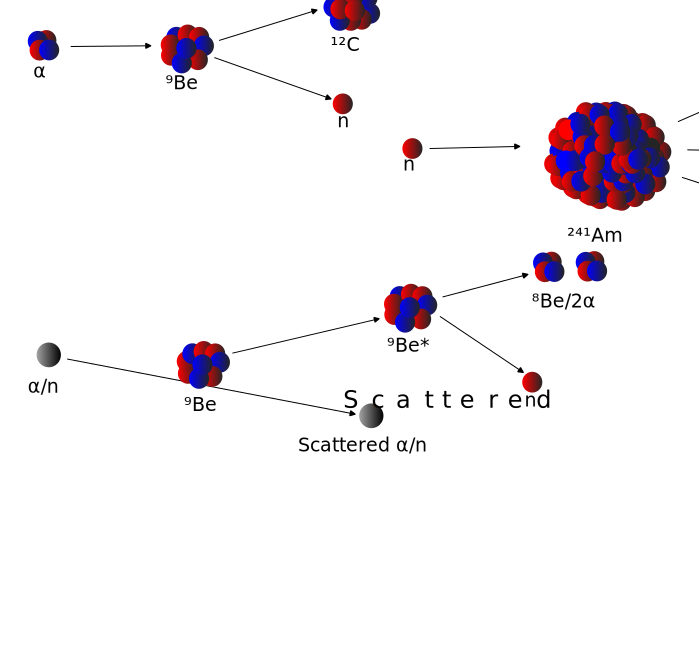
\includegraphics[width=\linewidth]{Fig4.1-AmBe-Processes-landscape}
%Explain processes, in particular break-up and fission (on average 3 neutrons)
%Don't talk about energy
%Join fast process with next slide
\end{frame}


\begin{frame}\frametitle{Fast reaction}
%Talk about carbon states populated and subsequent gammas being emitted
%These kinematically map to 3 regions
%n0,n1,n2 refer to carbon state
\begin{columns}[T]
\begin{column}{0.7\textwidth}
	\centering
	\vspace{-8pt}
	\includegraphics[width=\linewidth]{Fig5.1-GVDZ_resampled.pdf}
AmBe neutron distribution per $^{12}\text{C}$ state [Geiger-Van Der Zwan 1975]
\end{column}
\begin{column}{0.3\textwidth}
	\centering
	\includegraphics[width=\linewidth]{Fig5.2-Levelsout.pdf}
	$^{12}\text{C}$ states - ground, $1^\text{st}$, $2^\text{nd}$ [NNDC]
\end{column}
\end{columns}
\end{frame}

\section*{Current Status}
\begin{frame}\frametitle{Current status}
\begin{itemize}
		\item Geant4 has built in example in extended/hadronic/NeutronSource
		\item Simulates $^{241}\text{Am}$ $\alpha$-decay
		\item Lacks differential\\cross sections and\\crucial features
\end{itemize}
	\vspace*{-1.5cm}
	\hspace*{4cm}
	\includegraphics[width=.75\textwidth]{Fig6.1-AmBe_G4Original.pdf}
Geant4 extended/hadronic/NeutronSource example
\centering
%In particular, missing signature peaks of AmBe source, i.e. present the 3.3MeV one, but 5,6.8,7.7 and shoulder at 9.5 is missing
\end{frame}

\section*{Primary Generator}
\begin{frame}\frametitle{Implementation}
Aim: make the simulation as accurate as possible while reducing inefficiencies
\begin{itemize}
	\item Simulate $n$ and $^{12}\text{C}$ directly\\
	High activity sources $\Rightarrow$ $2.27\times10^6$ fast neutrons/s/Ci\\
	Simulate one fast neutron per event vs one neutron every $\approx~17000$ events using $\alpha$ decay method
	\item Rejection sampling techniques%iteratively generate randomised data and accept those within our defined XS and diff XS distributions
	\item Integrated and differential cross section from 1970 and 1975 Geiger and Van Der Zwan for $^{9}\text{Be}(\alpha,n)^{12}\text{C}$
	
\end{itemize}
~\newline
	%How does it work?say geant doesn't have diff Xs, we do.
%Rejection sampling is good
\end{frame}


%\begin{frame}\frametitle{Kinematic Lines}
%--What is XS and diff XS? Show difference between XS and diff XS, maybe a snapshot of the adopted data?
%--Kinematic lines are enough to show this
%
% Here showing kinematic lines for the first two states of carbon, clearly showing the angular dependence of the energy of the two reaction products
%\begin{columns}
%	\begin{column}[b]{0.5\linewidth}
%		\vspace*{-1cm}
%		\centering
%		\includegraphics[width=1\linewidth]{9BeA-12Cn-n0.png}
%		\centering
%		\includegraphics[width=\linewidth]{9BeA-12Cn-n2.png}
%	\end{column}
%	\begin{column}[b]{0.5\linewidth}
%		\centering
%		\includegraphics[width=1\linewidth]{9BeA-12Cn-n1.png}
%	\end{column}
%\end{columns}
%\end{frame}


\begin{frame}\frametitle{Differential cross-section contribution}
	%Anisotropical approach proposed in 1960s, works pretty well
	\begin{columns}
		\begin{column}[b]{0.5\linewidth}
			\centering
			\includegraphics[width=\textwidth]{Fig8.1-AmBeInitialNeutrons100s_isotropic}
			Initial neutrons: without differential cross-sections model
		\end{column}
		\begin{column}[b]{0.5\linewidth}
			\centering
			\includegraphics[width=\textwidth]{Fig8.2-AmBeInitialNeutrons100s_anisotropic}
			Initial neutrons: with differential cross-sections model
		\end{column}
	\end{columns}
\end{frame}


\begin{frame}\frametitle{Disadvantages}
%NOTE: D is diffusion coefficient, good to know but closely related to the diffusion length via the macroscopic absorbtion cross section
\begin{minipage}{\textwidth}
	Differential and Integrated cross section of beryllium-9 break-up not available
	\begin{itemize}
		\item $^{9}\text{Be}(\alpha,\alpha')$ scattering
		\item $^{9}\text{Be}^*$ angular decay information
		\item Other break-up channels more suppressed at interaction energy ($<5$~MeV)\\e.g. $^{9}\text{Be}^* \rightarrow\alpha+ ^{5}\text{He}$
	\end{itemize}
\end{minipage}  
\begin{minipage}{\textwidth}
	\includegraphics[width=\linewidth]{Fig9.1-AmBe-BreakUpProcesses.png}
\end{minipage}  
\end{frame}


\section*{Emerging Neutrons}

\begin{frame}\frametitle{Simulation Results - Emerging Neutrons}
	\centering
	Neutrons emerging from source casing (simulation)
	\centering
	\includegraphics[width=0.9\linewidth]{EmergingNeutrons20250402.png}
\end{frame}


\begin{frame}\frametitle{Simulation Results - Fission and Break-up Neutrons}
%Watt-fissiom distribution correctly shown
%Q value>200~MeV
%fission products being created up to 22~MeV
	\centering
	Fission and break-up neutrons emerging from the source material
	\centering
	\includegraphics[width=0.9\linewidth]{Fig10-Secondaries_20251020}
%
%produced inside the source
%Wendt-fission distribution,
%production up to 22 MeV
%Q values up to 200~MeV
%
\end{frame}


\begin{frame}\frametitle{Simulation Results - AmBe secondary $\gamma$s}
%DONE: TODO: replace with Carbon plot run without water
	\centering
	Secondary $\gamma$ produced per event ~~---~~ $^{241}\text{Am}$ $\gamma$ disabled to increase efficiency
	\centering
	\includegraphics[width=0.9\linewidth]{secondaryGammasEmerging}
\end{frame}

\section*{Model Comparison}
\begin{frame}\frametitle{Model comparison}
%Hoover quickly over shapes and features
%Don't say you have no idea why 7 MeV lower (n0 region)
%spend 2-3 minutes on this
%highlight differences in region,
%mention meas are correct
%good similarity to iso8529-1
	\centering
	Comparison with AmBe standards
	\centering
	\includegraphics[width=.9\linewidth]{Fig13-OverlapLine}
\end{frame}

\begin{frame}\frametitle{Comparison with Geant4 NeutronSource example}
	\includegraphics[width=0.9\linewidth]{EmergingNeutronsvsGeant.pdf}
\end{frame}

\section*{Conclusion}
\begin{frame}\frametitle{Conclusion}
\begin{itemize}
\item Validated AmBe neutron spectrum in Geant4
\item Correctly reproduced AmBe signature peaks
\item Implemented 1970 and 1975 Geiger-Van Der Zwan Cross sections (not otherwise present in Geant)
\item Faster execution than full $^{241}\text{Am}$ $\alpha$-decay chain recreation
\item Useful for analysis of flux and neutron moderation in various media
\item Future analysis of neutron moderation in water bath
%TODO: talk about so what, what to do with this now. Why is this useful
\end{itemize}
\centering
~\\Thank you for listening
\end{frame}


\section*{}%Backup slides
\appendix
\begin{frame}
~
Backup Slides
\end{frame}

\begin{frame}\frametitle{Primary Generator flowchart}
	\centering
	\includegraphics[width=0.7\linewidth]{FigBackup-PrimaryGenerator-v4-crop}
\end{frame}

%TODO!!!!! split slide 9 before and after theory
\begin{frame}\frametitle{Investigation of water bath}
	%AmBe source at centre of 1~m tall, 1~m diameter water tank.\\Fast neutrons are moderated by water. But what is actually happening here?\\
	%\begin{itemize}
	%	\item Mimic neutron moderation in a nuclear reactor
	%	\item Neutron activate samples for undergraduate forensic experiments
	%\end{itemize}
	\begin{itemize}
		\item Source neutron spectrum is known
		\item Source is at centre of 1~m tall, 1~m diameter water tank. The moderation profile is unknown
	\end{itemize}
	%In particular, experimental results from undergraduates disagree with the theroetical data [Lamar Baratta]
\end{frame}

\begin{frame}\frametitle{Two group model}
	Does it actually agree with the two-group neutron moderation model?
	\begin{columns}[T]
		\begin{column}{0.5\textwidth}
			Two group model:
			\[ \Phi_T = \frac{SL_T^2}{4\pi r \overline{D}(L_T^2-\tau_T)}(e^{-r/L_T}-e^{-r/\sqrt{\tau_T}}) \]
			describes thermal neutron diffusion and fast to thermal neutron moderation.\\
			\begin{itemize}
				\item $\tau_T\rightarrow$ (Fast) neutron age
				\item $L_t\rightarrow$ Thermal diffusion length
			\end{itemize}
		\end{column}
		\begin{column}{0.5\textwidth}
			\centering
			\includegraphics[width=\linewidth]{FigBackup-NeutronModeration}
			Neutron moderation $L^2=\frac{1}{6}\overline{r^2}$ [Lamarsh-Baratta 2001]
		\end{column}
	\end{columns}
\end{frame}

\begin{frame}\frametitle{Equivalent Dose - Preliminary}
	Calculated dose for outgoing $\gamma$ and neutrons from the water bath and verified against experimental\\
	Sampling over 0.2~s spectrum
	\begin{table}
		\centering
		\begin{tabular}{|c|c|c|}
			\hline
			Particle & Experimental [$\mu\text{Sv/h}$] &  Simulated [$\mu\text{Sv/h}$]\\
			\hline
			$\gamma$ & 1.54 & 8.05 \\
			\hline
			n & 0.8 & 1.68 \\
			\hline
		\end{tabular}
	\end{table}
	Notes:
	\begin{itemize}
		\item Neutrons measured with Nuclear Enterprises NM-2 dose monitor ($BF_3$)
		\item Gammas measured with dose monitor calibrated in the 59-1332~keV range
	\end{itemize}
\end{frame}


\end{document}
